% begin module greatest-integer-function
\begin{frame}
\begin{definition}[Greatest Integer Function]
The greatest integer function $[[x]]$ is defined by $[[x]] =$ the largest integer that is less than or equal to $x$.
\end{definition}
\begin{columns}[c]
\column{.5\textwidth}
\ 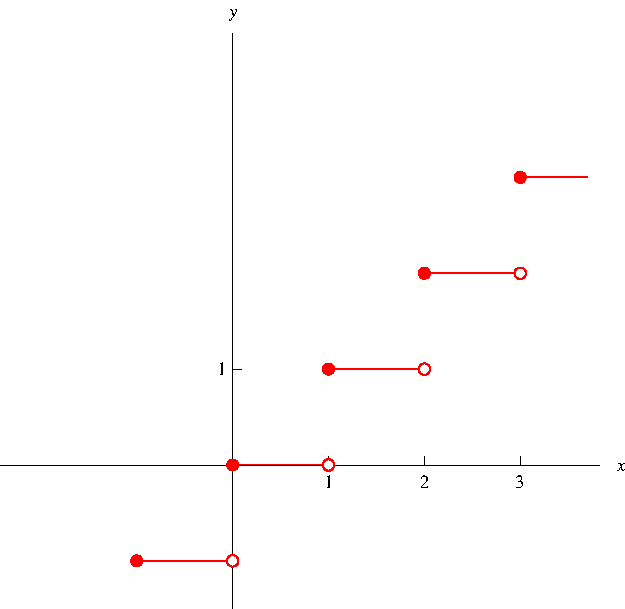
\includegraphics[height=4.5cm]{continuity/pictures/02-05-ex2d.pdf}%
\column{.5\textwidth}
\begin{align*}
\uncover<2->{%
\alert<handout:0| 2-3>{%
[[%
4%
]]%
}}%
& \uncover<2->{%
\alert<handout:0| 2-3>{%
 = \uncover<handout:0| 3->{%
 4%
}}}\\%
\uncover<2->{%
\alert<handout:0| 4-5>{%
[[%
4.8%
]]%
}}%
& \uncover<2->{%
\alert<handout:0| 4-5>{%
 = \uncover<handout:0| 5->{%
 4%
}}}\\%
\uncover<2->{%
\alert<handout:0| 6-7>{%
[[%
\pi%
]]%
}}%
& \uncover<2->{%
\alert<handout:0| 6-7>{%
 = \uncover<handout:0| 7->{%
 3%
}}}\\%
\uncover<2->{%
\alert<handout:0| 8-9>{%
[[%
\sqrt{2}%
]]%
}}%
& \uncover<2->{%
\alert<handout:0| 8-9>{%
 = \uncover<handout:0| 9->{%
 1%
}}}\\%
\uncover<2->{%
\alert<handout:0| 10-11>{%
\left[\left[%
-\frac{1}{2}%
\right]\right]%
}}%
& \uncover<2->{%
\alert<handout:0| 10-11>{%
 = \uncover<handout:0| 11->{%
-1%
}}}%
\end{align*}
\end{columns}
\end{frame}
% end module greatest-integer-function
